% 中期报告（参考学长案例格式）
% 基于 AI 的电网设备损伤检测与 SaaS 化设计
\documentclass[12pt,a4paper]{article}
\usepackage[UTF8]{ctex}
\usepackage{graphicx}
\usepackage{booktabs}
\usepackage{amsmath}
\usepackage{caption}
\usepackage{float}
\usepackage{hyperref}
\usepackage{geometry}
\geometry{left=2.5cm,right=2.5cm,top=2.5cm,bottom=2.5cm}

\title{基于 AI 的电网设备损伤检测与 SaaS 化设计\\中期报告}
\author{冯宇捷\\指导教师：侯金}
\date{\today}

\begin{document}
\maketitle

\begin{abstract}
本报告为“基于 AI 的电网设备损伤检测与 SaaS 化设计”课题的中期总结。电力设备在运行中面临鸟巢、渗漏油、局部过热等典型损伤，传统人工巡检成本高、风险大且难以全覆盖。本项目旨在构建可扩展的 SaaS 化巡检平台：以多模态数据（无人机可见光、红外、传感器与历史记录）为输入，通过 AI 进行损伤检测与识别，并输出告警、工单与可视化分析。中期阶段已完成模块 A（鸟巢检测）端到端 PoC、模块 B（漏油检测）训练与部署、模块 C（红外高温检测）在 Flask 中的实现与接入（支持自定义温度区间、OCR 识别温区、水印干扰去除等）；报告总结了技术路线、已完成工作、存在问题与下一步计划。
\end{abstract}

\tableofcontents
\newpage

%=============================================================================
\section{毕业设计（论文）概述}
%=============================================================================

\subsection{背景与目标}

电力设备在运行中易出现鸟巢、渗漏油、局部过热等损伤，传统人工巡检效率低、风险高且难以全覆盖。本项目旨在构建可扩展的 SaaS 化巡检平台：以多模态数据（无人机可见光、红外、传感器与历史记录）为输入，通过 AI 进行损伤检测与识别，输出告警、工单与可视化分析；采用统一认证、多租户隔离与模型注册的 SaaS 设计，便于多部门共用同一套检测能力并与告警中心、工单系统对接。中期阶段已完成模块 A（鸟巢）端到端 PoC、模块 B（漏油）训练与部署、模块 C（红外高温）在 Flask 中的实现与接入。

\subsection{研究内容与技术路线}

采用“垂直切片、横向扩展”策略：先完成单模块从数据到部署的完整链路，再建设多模块注册与统一调度。技术路线：（1）\textbf{数据}：鸟巢 COCO、漏油 VOC/YOLO，脚本生成训练/验证集，增强与预处理在训练管线内完成；（2）\textbf{训练}：鸟巢 Mask R-CNN 实例分割，漏油 YOLOv8 目标检测，统一 AMP、学习率调度与 DataLoader 优化；（3）\textbf{部署}：Flask 微服务提供 REST API、批量上传与推理，鸟巢/漏油/红外三模块均已接入。鸟巢选 Mask R-CNN 以同时输出框与掩码便于与工单关联，漏油选 YOLOv8 兼顾速度与框级定位需求。

\subsection{模块规划}

\begin{itemize}
  \item \textbf{Module A（鸟巢检测）}：已完成 PoC，验证整条管线（数据—训练—部署）。
  \item \textbf{Module B（漏油检测）}：已在 CSDN 数据集（train10-csdn）上完成 YOLOv8s 训练并接入 Flask；验证集最佳 mAP50 约 0.39，mAP50-95 约 0.26，详见第三部分。
  \item \textbf{Module C（红外高温检测）}：已实现并接入 \texttt{deploy/flask-service}，支持用户自定义告警温度区间、OCR 识别图像高低温刻度、水印与图例干扰去除，详见第三部分。
\end{itemize}

%=============================================================================
\section{毕业设计（论文）整体安排及进度}
%=============================================================================

整体安排及进度与开题报告一致，采用“双线并进”的阶段性规划（可参考《冯宇捷交大开题报告》中的进度表与甘特图）。各阶段划分如下。

\subsection{进度阶段划分}

\begin{itemize}
  \item \textbf{第 1--4 周（已完成）：} 模块 A（鸟巢检测）PoC 实现：数据准备、Mask R-CNN 训练、工程优化与 Flask 微服务部署，完成从数据到可调用服务的垂直切片验证。
  \item \textbf{第 5--10 周：} Track 1 —— SaaS 平台建设。建立多租户后端、RBAC、任务编排与 AI 模型注册表 API，并将 PoC 训练工具产品化。
  \item \textbf{第 11--18 周：} Track 2 —— 新模块扩展。模块 C（红外）已接入；完成模块 B（漏油）的完整训练与指标记录，复用平台数据处理与训练能力，巩固三模块在注册表与微服务目录中的集成。
  \item \textbf{第 19--20 周：} 最终集成与答辩。多模块与多用户端到端测试、系统优化、最终报告撰写与答辩准备。
\end{itemize}

\subsection{时间安排说明}

上述安排与开题答辩中的 Work Plan 一致：先完成单模块垂直切片（模块 A），再横向扩展平台能力（Track 1）与新模块（Track 2），最后集中完成集成与论文。若开题报告中另有更细的周次或里程碑划分，以开题报告为准进行对照与更新。

% 若存在甘特图，可取消下面注释以插入（与开题报告进度一致）
% \begin{figure}[H]
%   \centering
%   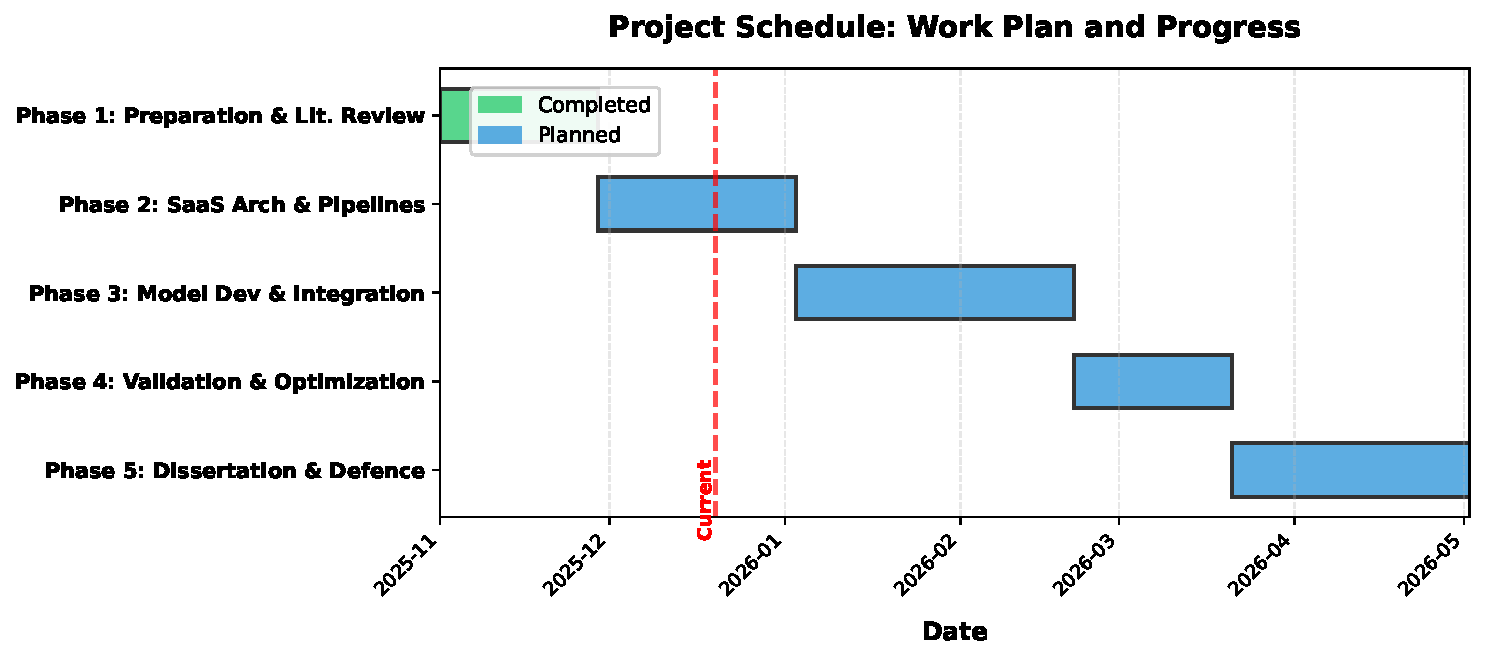
\includegraphics[width=0.9\textwidth]{../../schedule/project_schedule_gantt_proposal.png}
%   \caption{毕业设计整体安排与进度（可与开题报告甘特图一致）。}
% \end{figure}

%=============================================================================
\section{毕业设计（论文）已完成的研究部分}
%=============================================================================

\subsection{模块 A：鸟巢检测 PoC}

\subsubsection{数据与增强}

使用 COCO 格式鸟巢数据集，共 54 张图像（43 张训练、11 张验证），每张图像包含鸟巢的边界框与实例分割多边形标注。采用确定性数据增强替代生成式方法（如 Stable Diffusion 等），原因在于前期尝试中发现生成式方法易产生物理不合理的伪影（如在不锈钢件上生成锈迹、纹理错位），影响模型对真实损伤的判别；确定性增强在保证几何与光度合理性的前提下，仍能显著增加样本多样性。具体包括：自定义 Random IoU Crop（尺度 0.3--1.0），迫使模型学习部分遮挡与多尺度目标；光度扰动（亮度、对比度等）模拟现场光照变化；ResizeMax 与 PadSquare 统一宽高比并固定输入尺寸。上述流程均基于 \texttt{torchvision.transforms.v2} 实现，与 PyTorch 2.x 及 DataLoader 兼容良好。

\subsubsection{模型与训练配置}

\begin{itemize}
  \item 模型：Mask R-CNN（ResNet50 + FPN v2），适用于实例分割与损伤区域精确定位。
  \item 输入尺寸：$512\times512$，batch size 4，epochs 40（支持 early stopping）。
  \item 优化器：AdamW，学习率 $5\times10^{-4}$，OneCycleLR 调度，混合精度（AMP）；单 epoch 约 27 秒，优化后 GPU 利用率约 70--85\%。
\end{itemize}

\subsubsection{验证指标与训练曲线}

COCO 验证集上：bbox AP$_{50}$ = 1.000，segm AP$_{50}$ = 1.000，segm AP$_{75}$ = 0.919，AR@[0.50:0.95] 约 0.83；训练损失由约 1.41 降至 0.14，验证损失由约 0.65 降至 0.19，约在第 20 轮后趋于平稳，未观察到明显过拟合。PR 曲线在 IoU=0.50 时精度接近 1.0，IoU 提高至 0.75、0.90 时略有下降，说明高 IoU 下对定位更敏感；IoU 分布右偏，得分阈值在 0.4--0.5 附近时 F1 较优，实际部署可据此调节置信度阈值以平衡漏检与误报。

\begin{figure}[H]
  \centering
  \includegraphics[width=0.85\textwidth]{../../../experiments/visualizations/loss_curves.png}
  \caption{鸟巢检测训练/验证损失曲线；约第 20 轮后趋于平稳。}
\end{figure}

\begin{figure}[H]
  \centering
  \includegraphics[width=0.85\textwidth]{../../../experiments/visualizations/pr_curve_bbox_ap50.png}
  \caption{鸟巢检测 bbox PR 曲线（IoU 0.50/0.75/0.90）。}
\end{figure}

\begin{figure}[H]
  \centering
  \includegraphics[width=0.85\textwidth]{../../../experiments/visualizations/iou_hist_bbox.png}
  \caption{鸟巢检测 bbox IoU 分布；右偏表明定位质量较好。}
\end{figure}

\begin{figure}[H]
  \centering
  \includegraphics[width=0.85\textwidth]{../../../experiments/visualizations/threshold_sweep_bbox.png}
  \caption{得分阈值与精确率/召回率/F1 关系（IoU$\geq$0.5）；阈值 0.4--0.5 附近 F1 较优。}
\end{figure}

\subsection{模块 B：漏油检测}

\subsubsection{数据准备}

漏油数据来自两路：一是原始 VOC 格式数据集（约 103 张，含 XML 标注）；二是来自 CSDN 等渠道的 YOLO 格式数据。通过 prepare\_dataset.py 支持三种模式：仅原始 VOC、仅 CSDN YOLO、以及合并两路数据（约 333 张，按约 8:2 划分训练/验证）。脚本将 VOC 框坐标转换为 YOLO 归一化格式，统一类别为 oil\_leak，并生成数据集 YAML 供 YOLOv8 直接读取。本次报告采用的训练结果来自 runs/detect/train10-csdn，该实验使用 \textbf{CSDN 数据集}（oil\_leak\_csdn.yaml），即仅使用 CSDN 渠道的 YOLO 格式数据。

\subsubsection{训练配置}

采用 YOLOv8s（yolov8s.pt），单类别检测。train10-csdn 主要超参数：epochs 150、输入 640、batch 8、AdamW、cos 学习率、mosaic 0.3、mixup 0.05、cache 使用 RAM、patience 30、AMP 开启，固定随机种子 42。训练脚本为 src/oil\_leak/train.py，可通过命令行指定 \texttt{--data}、\texttt{--epochs}、\texttt{--model} 等。

\subsubsection{验证指标与训练结果}

train10-csdn 共训练 123 个 epoch，验证集上最佳指标出现在第 93--94 轮附近：\textbf{precision(B)} 约 0.83、\textbf{recall(B)} 约 0.34、\textbf{mAP50(B)} 约 0.39、\textbf{mAP50-95(B)} 约 0.26。训练损失（box/cls/dfl）随 epoch 逐步下降并趋于稳定。图\,\ref{fig:oil-pr}、图\,\ref{fig:oil-f1} 与图\,\ref{fig:oil-cm} 分别为验证集 PR 曲线、F1 曲线与归一化混淆矩阵；可将该次训练得到的最佳权重（best.pt）拷贝为 checkpoints/oil\_leak\_yolov8.pt 供 Flask 推理服务加载。

\begin{figure}[H]
  \centering
  \includegraphics[width=0.85\textwidth]{../../../src/oil_leak/runs/detect/train10-csdn/BoxPR_curve.png}
  \caption{漏油检测（train10-csdn）验证集精确率-召回率曲线；IoU 阈值 0.5。}
  \label{fig:oil-pr}
\end{figure}

\begin{figure}[H]
  \centering
  \includegraphics[width=0.85\textwidth]{../../../src/oil_leak/runs/detect/train10-csdn/BoxF1_curve.png}
  \caption{漏油检测（train10-csdn）验证集 F1 曲线；不同置信度阈值下的 F1 分数。}
  \label{fig:oil-f1}
\end{figure}

\begin{figure}[H]
  \centering
  \includegraphics[width=0.7\textwidth]{../../../src/oil_leak/runs/detect/train10-csdn/confusion_matrix_normalized.png}
  \caption{漏油检测（train10-csdn）验证集归一化混淆矩阵。}
  \label{fig:oil-cm}
\end{figure}

\subsubsection{与 Flask 服务集成}

Flask 推理服务已支持“漏油检测”模型：根据模型注册表中的 \texttt{weights\_path} 加载 YOLOv8 权重，对上传图像执行推理，返回检测框坐标、置信度与可视化叠加图；若注册表路径缺失或文件不存在，服务会回退到 \texttt{checkpoints/oil\_leak\_yolov8.pt}，保证在权重尚未迁移到数据库时仍可正常使用。漏油模块与鸟巢模块共用同一套上传、推理与下载接口，仅根据用户选择的模型类型切换后端实现，便于后续在统一前端中扩展更多检测模块。

\subsection{SaaS 部署与 Flask 微服务}

\subsubsection{功能概述}

部署于 \texttt{deploy/flask-service}，提供以下能力：

\begin{itemize}
  \item 批量图像上传与实时推理：用户可选择“鸟巢检测”“漏油检测”或“红外高温检测”等已注册模型，上传单张或多张图像，服务端按模型类型调用对应推理逻辑（Mask R-CNN、YOLOv8 或红外混合检测），返回 JSON 格式的检测框、置信度/温度及类别，并生成叠加了框与掩码的可视化图。
  \item 单张与 ZIP 结果下载：支持单张结果图下载及批量结果打包为 ZIP，便于现场巡检后离线查看与归档。
  \item 统计看板与图表：对历史推理任务与检测结果进行汇总展示，便于了解各模型调用情况与告警分布。
  \item 大图内存优化与错误处理：对大尺寸输入进行 resize 或分块策略，避免 OOM；接口层对异常进行捕获并返回明确错误信息，保证服务稳定可用。
\end{itemize}

\subsubsection{接口与运行方式}

请求流程为：用户通过 Web 页面上传图像并选择模型 $\rightarrow$ 服务根据模型类型解析权重路径并执行推理 $\rightarrow$ 返回结构化结果与可视化图 URL。开发环境运行方式：\texttt{python run.py}，默认监听 \texttt{0.0.0.0:5000}；生产环境建议使用 Gunicorn 多进程（如 \texttt{gunicorn -w 4 wsgi:app}），以提升并发能力。

\subsubsection{平台意义}

作为“模型即服务”的落地，鸟巢、漏油与红外高温三模块均已通过统一接口对外提供推理能力；模型注册表与权重路径的配置化设计为多租户 SaaS、RBAC 与任务编排预留了架构空间。

\subsection{模块 C（红外高温检测）}

红外高温检测已在 deploy/flask-service 中实现并接入，与鸟巢、漏油共用同一套上传、推理与下载接口。实现位于 app/services/model\_service.py 与 app/routes/inference.py，采用 OCR 与像素映射的混合方案，无需单独训练深度学习模型即可对红外热力图进行高温区域检测。

主要功能包括：(1) 用户自定义告警温度区间：前端或 API 传入告警温度阈值（默认 50$^\circ$C），服务据此将灰度映射为温度并筛选超过阈值的热点区域。(2) OCR 识别高低温刻度：使用 EasyOCR 对红外图像进行文字检测与识别，从图例或刻度区域解析出图像对应的最高温与最低温，用于将像素灰度线性映射到温度值，并对常见 OCR 误识别做启发式修正。(3) 去除水印与图例干扰：通过边框水印掩码构建函数检测并掩码图像边缘的白色水印与 Logo 区域，避免被误判为高温热点；通过 OCR 文本区域掩码排除图例与刻度数字，减少误检。输出包括热点框、每个热点的温度值、全图最大读取温度与最大热点温度，以及叠加了框与温度标注的可视化图。

% 若存在 reports/defense/assets 下的截图，可取消下面注释以插入
% \begin{figure}[H]
%   \centering
%   \includegraphics[width=0.75\textwidth]{../../assets/flask-deploy-image.png}
%   \caption{Flask 服务批量检测界面；支持多图上传与模型选择。}
% \end{figure}

%=============================================================================
\section{下一部分的工作安排}
%=============================================================================

\subsection{Track 1：SaaS 平台（约第 4--10 周）}

\begin{itemize}
  \item 实现多租户后端、RBAC 与任务编排：包括用户/角色/权限的数据模型与接口设计、任务队列（如 Celery 或内存队列）与任务状态查询，使多用户可并发提交检测任务并查看结果。
  \item 定义 AI 模型注册表 API：统一模型的注册、查询、启用/停用及权重路径管理，便于前端与调度层按名称或类型选择模型，并为后续模型版本与 A/B 测试留接口。
  \item 将 PoC 训练工具（增强、日志等）产品化：把当前脚本中的增强配置、训练日志与 checkpoint 管理抽象为可配置、可复用的工具，供漏油与红外模块共用，减少重复开发。
\end{itemize}

\subsection{Track 2：新模块扩展（约第 11--18 周）}

\begin{itemize}
  \item 推进模块 B（漏油）的完整实验与巩固模块 C（红外）：完成漏油在合并数据集上的完整训练与验证指标记录并更新注册表；红外模块已上线，后续可做鲁棒性优化与多设备红外图适配。
  \item 复用平台的数据处理与训练能力：新模块尽量复用 \texttt{prepare\_dataset}、训练脚本与部署管线，仅替换数据路径与模型类型，降低维护成本。
  \item 将新模块接入注册表与微服务目录：在数据库与前端中增加新模型条目，确保任务路由与推理逻辑能正确识别并调用。
\end{itemize}

\subsection{收尾与答辩（约第 19--20 周）}

最终集成、系统测试与报告撰写：对多模块、多用户场景做端到端测试，整理实验数据与截图，完成最终报告与答辩材料；预期产出包括可演示的鸟巢/漏油/红外三模块 SaaS 原型、符合要求的书面报告与答辩展示。

%=============================================================================
\section{毕业设计（论文）工作中存在的问题}
%=============================================================================

\subsection{泛化能力}

当前鸟巢验证集上 AP$_{50}$=1.0、IoU 接近 1.0，与训练场景高度一致，说明在“与训练同分布”的验证集上模型表现良好。但在实际复杂场景（雾霾、逆光、新杆型、不同季节与地域）下，性能可能明显下降。因此，数据增强、负样本构建与多场景评估是平台级共性需求：后续计划引入更多跨场景数据或留出一批“未参与训练”的现场数据做泛化测试，并在漏油与红外模块中同样重视负样本与困难样本设计，避免仅在小规模、同分布数据上追求过高指标而忽视真实场景鲁棒性。

\subsection{技术选型讨论}

\begin{itemize}
  \item \textbf{SaaS 后端}：是优先做功能完整的原型（如简易 RBAC、任务队列与多租户隔离的雏形）还是从第一天就投入生产级认证（如 OAuth2、审计日志），需结合课题时间与答辩目标权衡；当前倾向先完成可演示的多模型、多任务原型，再视时间补充权限与审计。
  \item \textbf{漏油模块}：漏油检测目前采用 YOLOv8 框级检测，已能满足“有无漏油与大致位置”的需求；若业务后续要求精确到油渍边界（如面积统计、趋势对比），可评估引入语义分割（如 U-Net）或与实例分割联合，届时需补充像素级标注数据。
  \item \textbf{红外模块}：红外高温检测已作为独立模块接入，支持自定义告警温度与 OCR 温区识别；后续可考虑与可见光融合做多模态分析（如 RGB+热力图联合输入），需结合现场数据与运维需求再定接口与模型结构。
\end{itemize}

\subsection{局限与风险}

当前数据规模仍偏小（鸟巢 54 张、漏油合并后约 333 张），标注质量与一致性对结果影响较大；部署环境上，Flask 单机多进程可支撑中小并发，若需更高并发或分布式推理，需进一步引入队列与 worker 池。这些将在后续阶段通过数据扩充与架构迭代逐步缓解。

%=============================================================================
\section{参考文献}
%=============================================================================

\begin{enumerate}
  \item He K, Gkioxari G, Dollár P, et al. Mask R-CNN[C]//ICCV, 2017.
  \item Lin T Y, Maire M, Belongie S, et al. Microsoft COCO: Common objects in context[C]//ECCV, 2014.
  \item Jocher G, et al. Ultralytics YOLOv8. \href{https://github.com/ultralytics/ultralytics}{github.com/ultralytics/ultralytics}
  \item Redmon J, Divvala S, Girshick R, et al. You only look once: Unified, real-time object detection[C]//CVPR, 2016.
  \item PyTorch. torchvision.models.detection. \href{https://pytorch.org/vision/stable/models.html}{pytorch.org/vision}
  \item Flask. Web framework. \href{https://flask.palletsprojects.com/}{flask.palletsprojects.com}
\end{enumerate}

\end{document}
